\subsubsection{Evaluation Session \& Progress Update}
\begin{figure}[H]
    \centering
    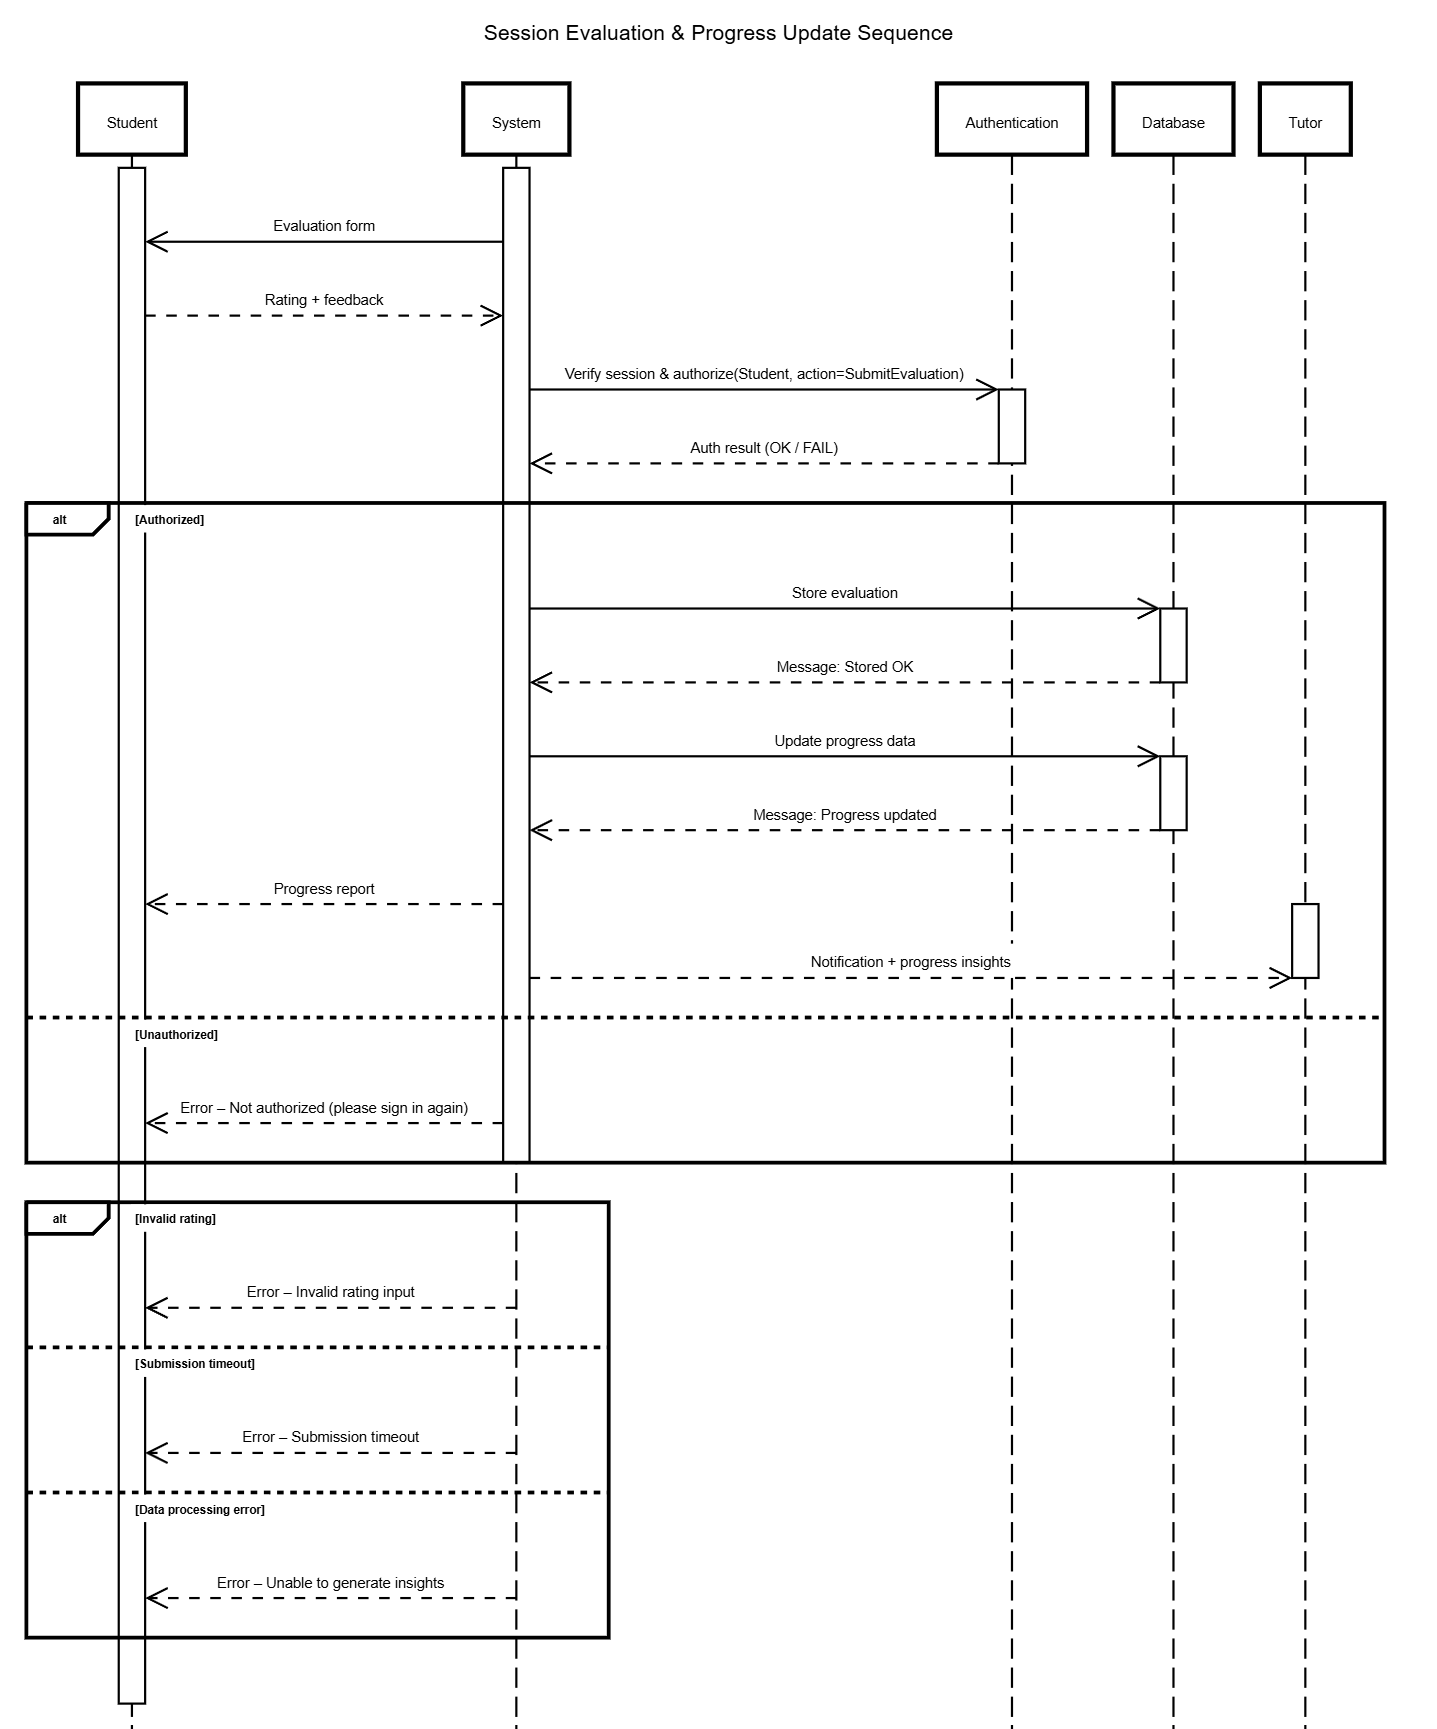
\includegraphics[width=0.8\textwidth]{graphics/chapter3/student/evaluation.png}
    \caption{Sequence diagram of Evaluating and Updating Progress}
    \label{fig:evaluation}
\end{figure}

\newpage
\noindent \textbf{Description} \\ 
\textbf{Actors:} Student, System, Database, Tutor

\begin{enumerate}
    \item System automatically sends evaluation form to student
    \item Student sends feedback to the system
    \item System requires a valid token in current session from student to access database
    \item If authenticated, system stores student's evaluation and updates progress
    \item Database returns messages of successful notifications
    \item At the time evaluation from student stored successfully, tutor is noticed by system to read this evaluation
    \item If interrupted in process of interaction between student and system, the system returns status code with a certain phrases: \texttt{Error + System Error Cause}
\end{enumerate}
